\section{(W) Moving obstacles, intruders, and constraints}\label{s:intruders}
    \noindent Fast overview of obstacles and space constraints which position is dynamic relative to mission or avoidance time frame:
    \begin{itemize}
        \item Non-cooperative intruders
        \item Short term bad weather areas (constraints)
        \item The models are based on \emph{analytical geometry} for \emph{cones and ellipsoids} taken from \cite{sommerville2016analytical}.
        \item The cell boundary was approximated as set of points, the intersection objects were discretized.
        \item Closes point problem \cite{shamos1975closest} was solved by application of method  \cite{bentley1980optimal}
		\item Moving obstacles were adressed in \cite{fiorini1998motion}.
		\item Lidar like intersection rebase the obstacle or intruder into pointcloud with evaluated impact rate ...
    \end{itemize}
    
\subsection{(W) Intruder behaviour prediction}\label{s:intruderBehaviourPrediction}
    \noindent Prediction of impact area in \emph{avoidance grid} based on available parameters:
    \begin{itemize}
        \item Intruder/Constraint position
        \item Intruder/Constraint velocity/heading
        \item Intruder movement certainty (Horizontal/Vertical maneuverability)
    \end{itemize}
    
\subsection{(W) Linear intersection model}\label{s:linearIntersectionModel}
    \noindent Prediction of \emph{impact area}, based on intruder position/velocity, usable for \emph{small body volume relative to average cell size}.
    
\subsection{(W) Body-volume intersection}\label{s:bodyvolumeIntersection}
    \noindent Prediction of \emph{impact area} based on intruder position/velocity/estimated body volume, mandatory for \emph{large scale objects} and \emph{Short term bad weather areas}.
    
\subsection{(W) Maneuverability uncertainty intersection}\label{s:uncertaintyIntersection}
    \noindent Prediction of \emph{impact area} based on intruder position/velocity/estimated maneuverability, usable for \emph{expected adversarial behaviour}. Intersection polytope volume calculation \cite{lawrence1991polytope}
    
    \begin{figure}[H]
    	\centering
        \begin{subfigure}{0.48\textwidth}
            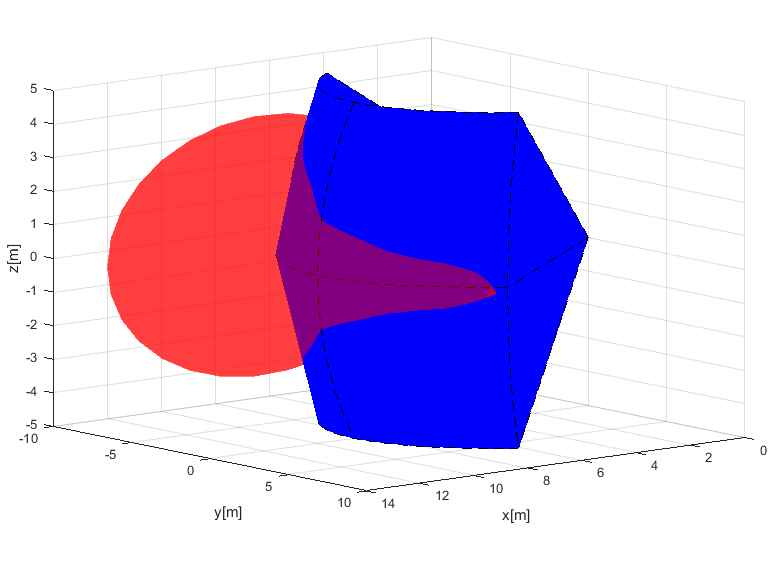
\includegraphics[width=0.9\linewidth]{\FIGDIR/TE013ElipticConeIntersecitonExample}
            \caption{\emph{Avoidance Grid} Intersection.}
            \label{fig:ellipticConeIntersectionExample}
        \end{subfigure}
        \begin{subfigure}{0.48\textwidth}
            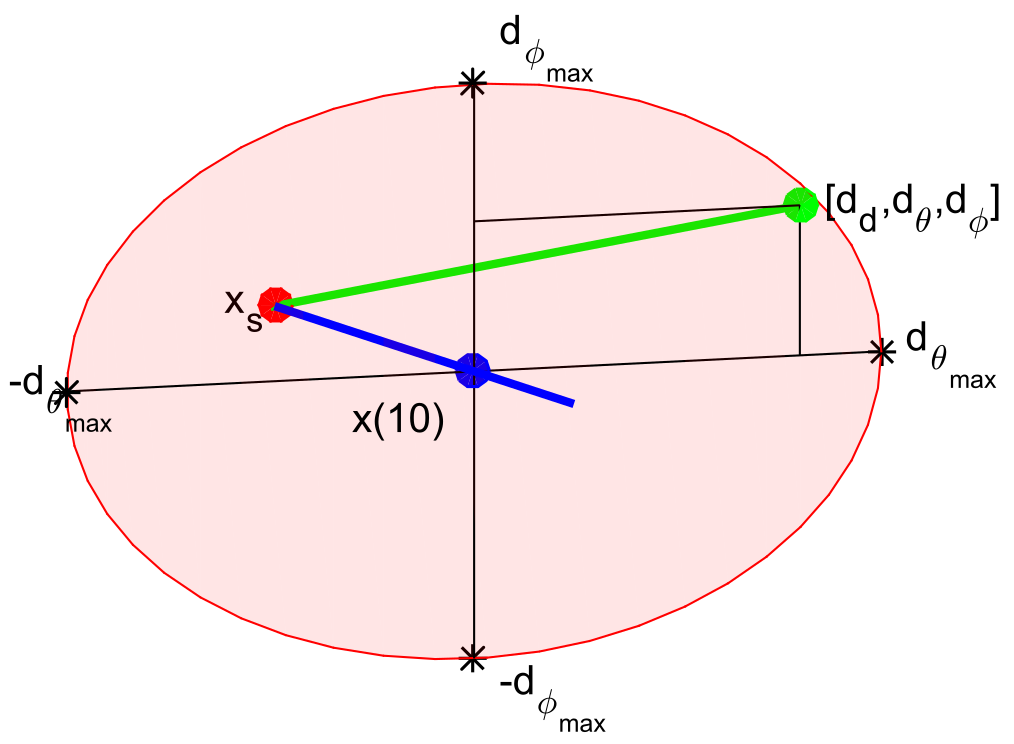
\includegraphics[width=0.9\linewidth]{\FIGDIR/TE014ElipticConeIOnePoint} 
            \caption{Horizontal slice.}
            \label{fig:ellipticalConeHorizontalSlice}
        \end{subfigure}
        \caption{Elliptical cone represented maneuverability approximation. }
        \label{fig:ellipticalConeRepresentedManuevurabilityApproximation}
    \end{figure}
    
    \begin{figure}[H]
    	\centering
        \begin{subfigure}{0.48\textwidth}
            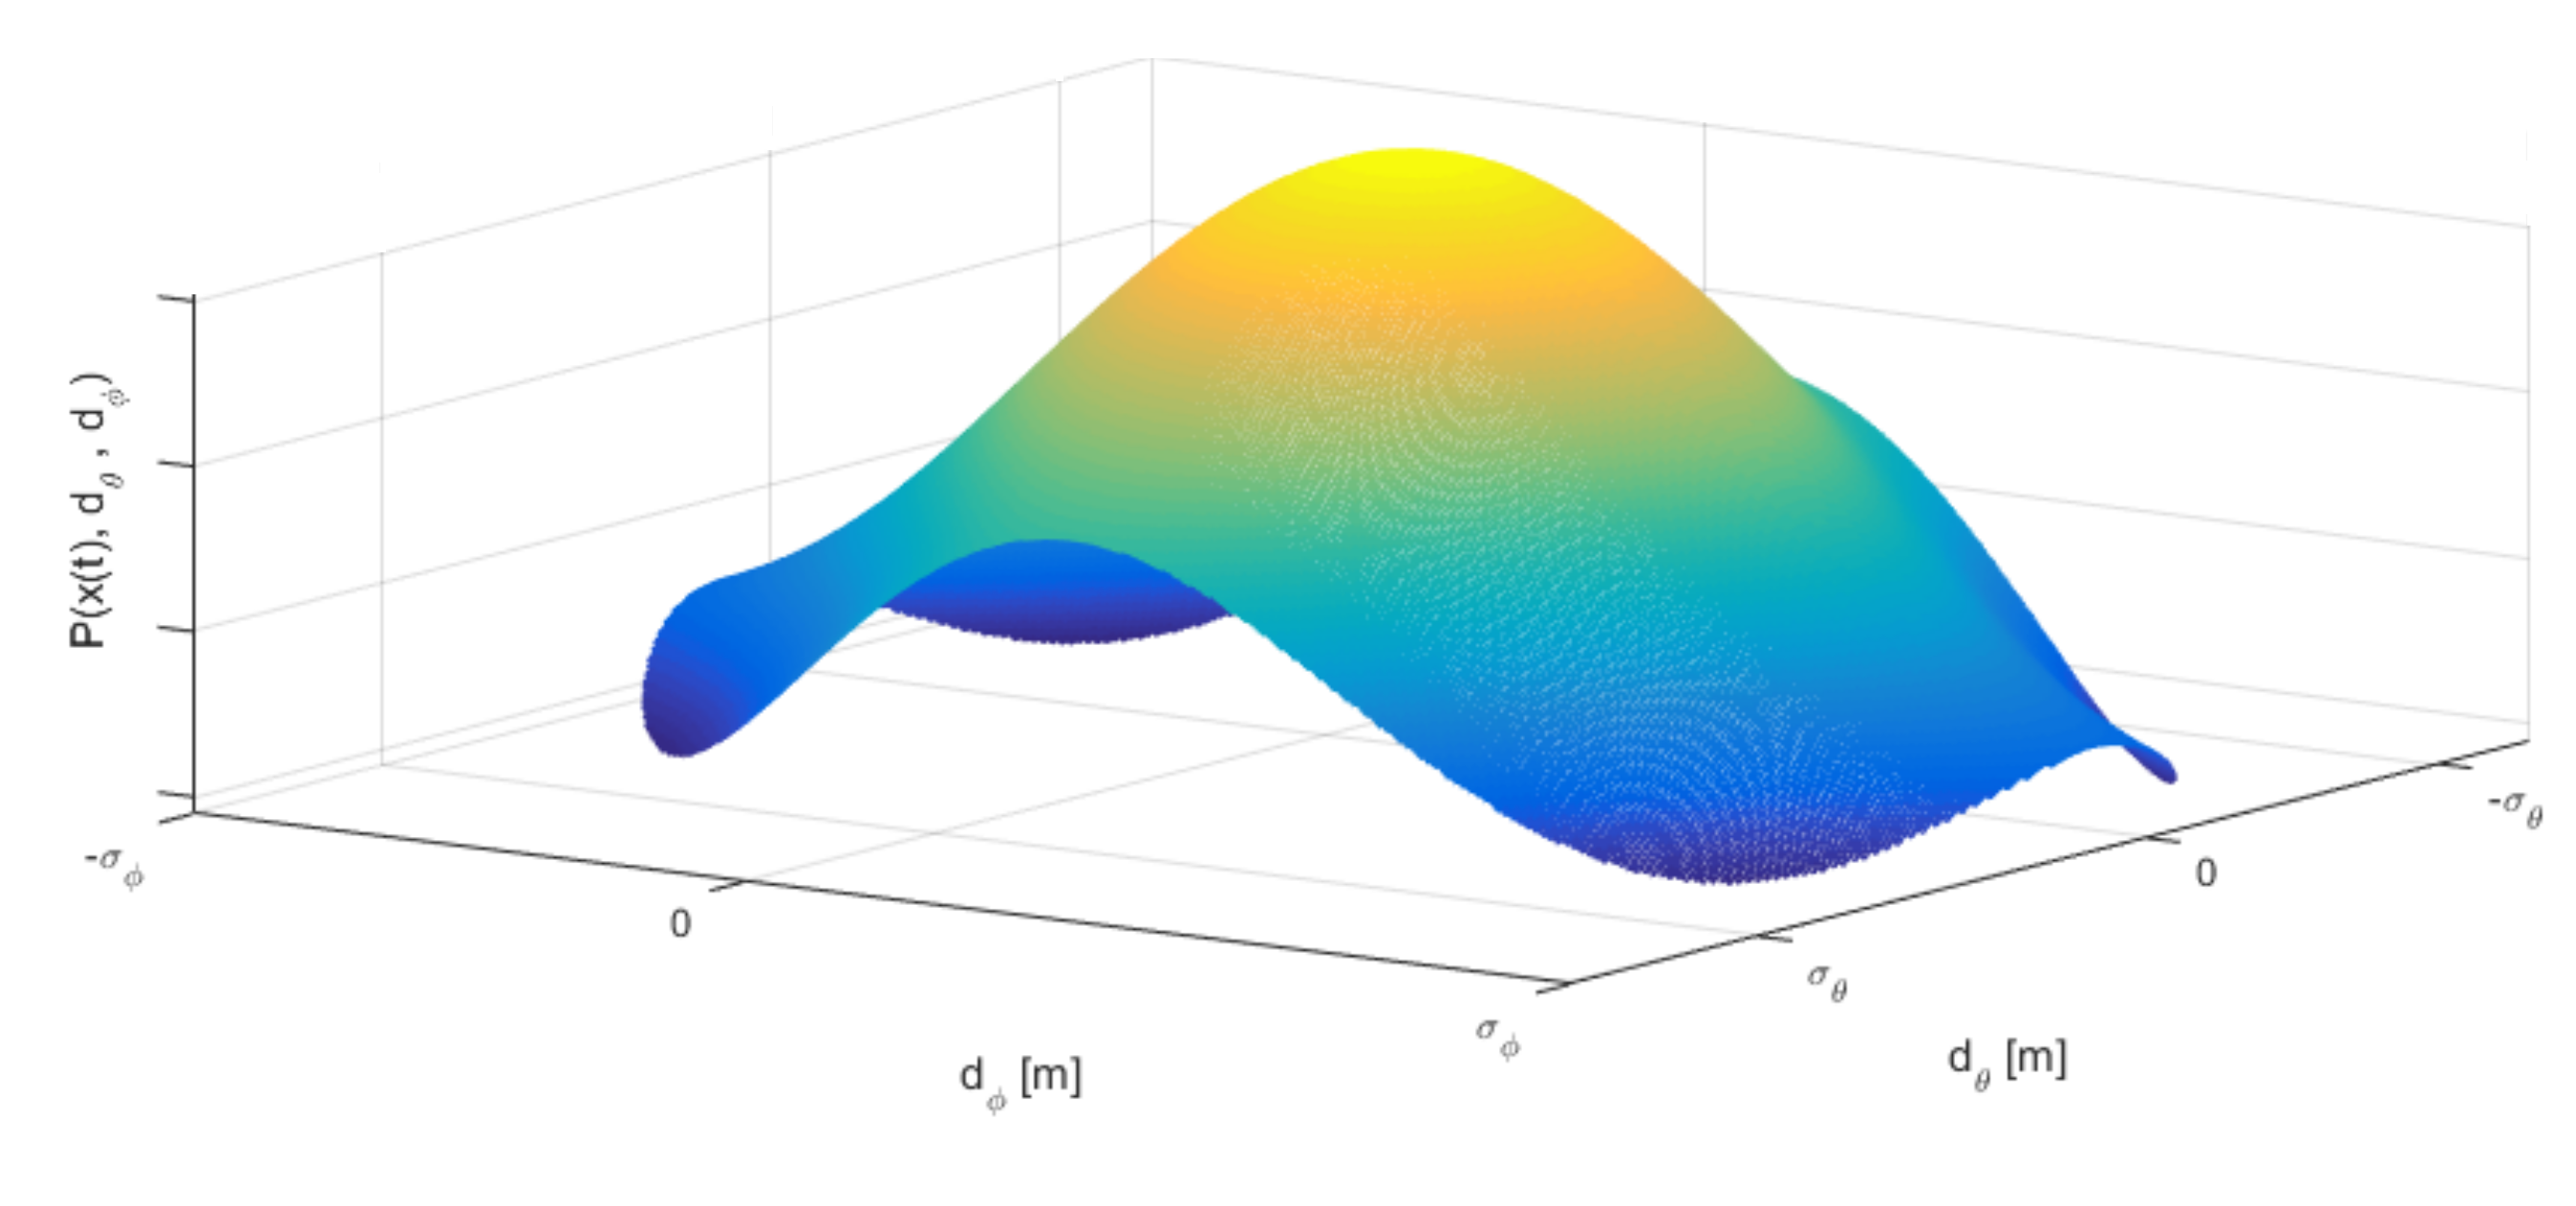
\includegraphics[width=0.9\linewidth]{\FIGDIR/TE015ProbabilisticDistributionOfEllipsoidCutSideForTE016}
            \caption{Intruder passing probability.}
            \label{fig:intruderPassingProbability}
        \end{subfigure}
        \begin{subfigure}{0.48\textwidth}
            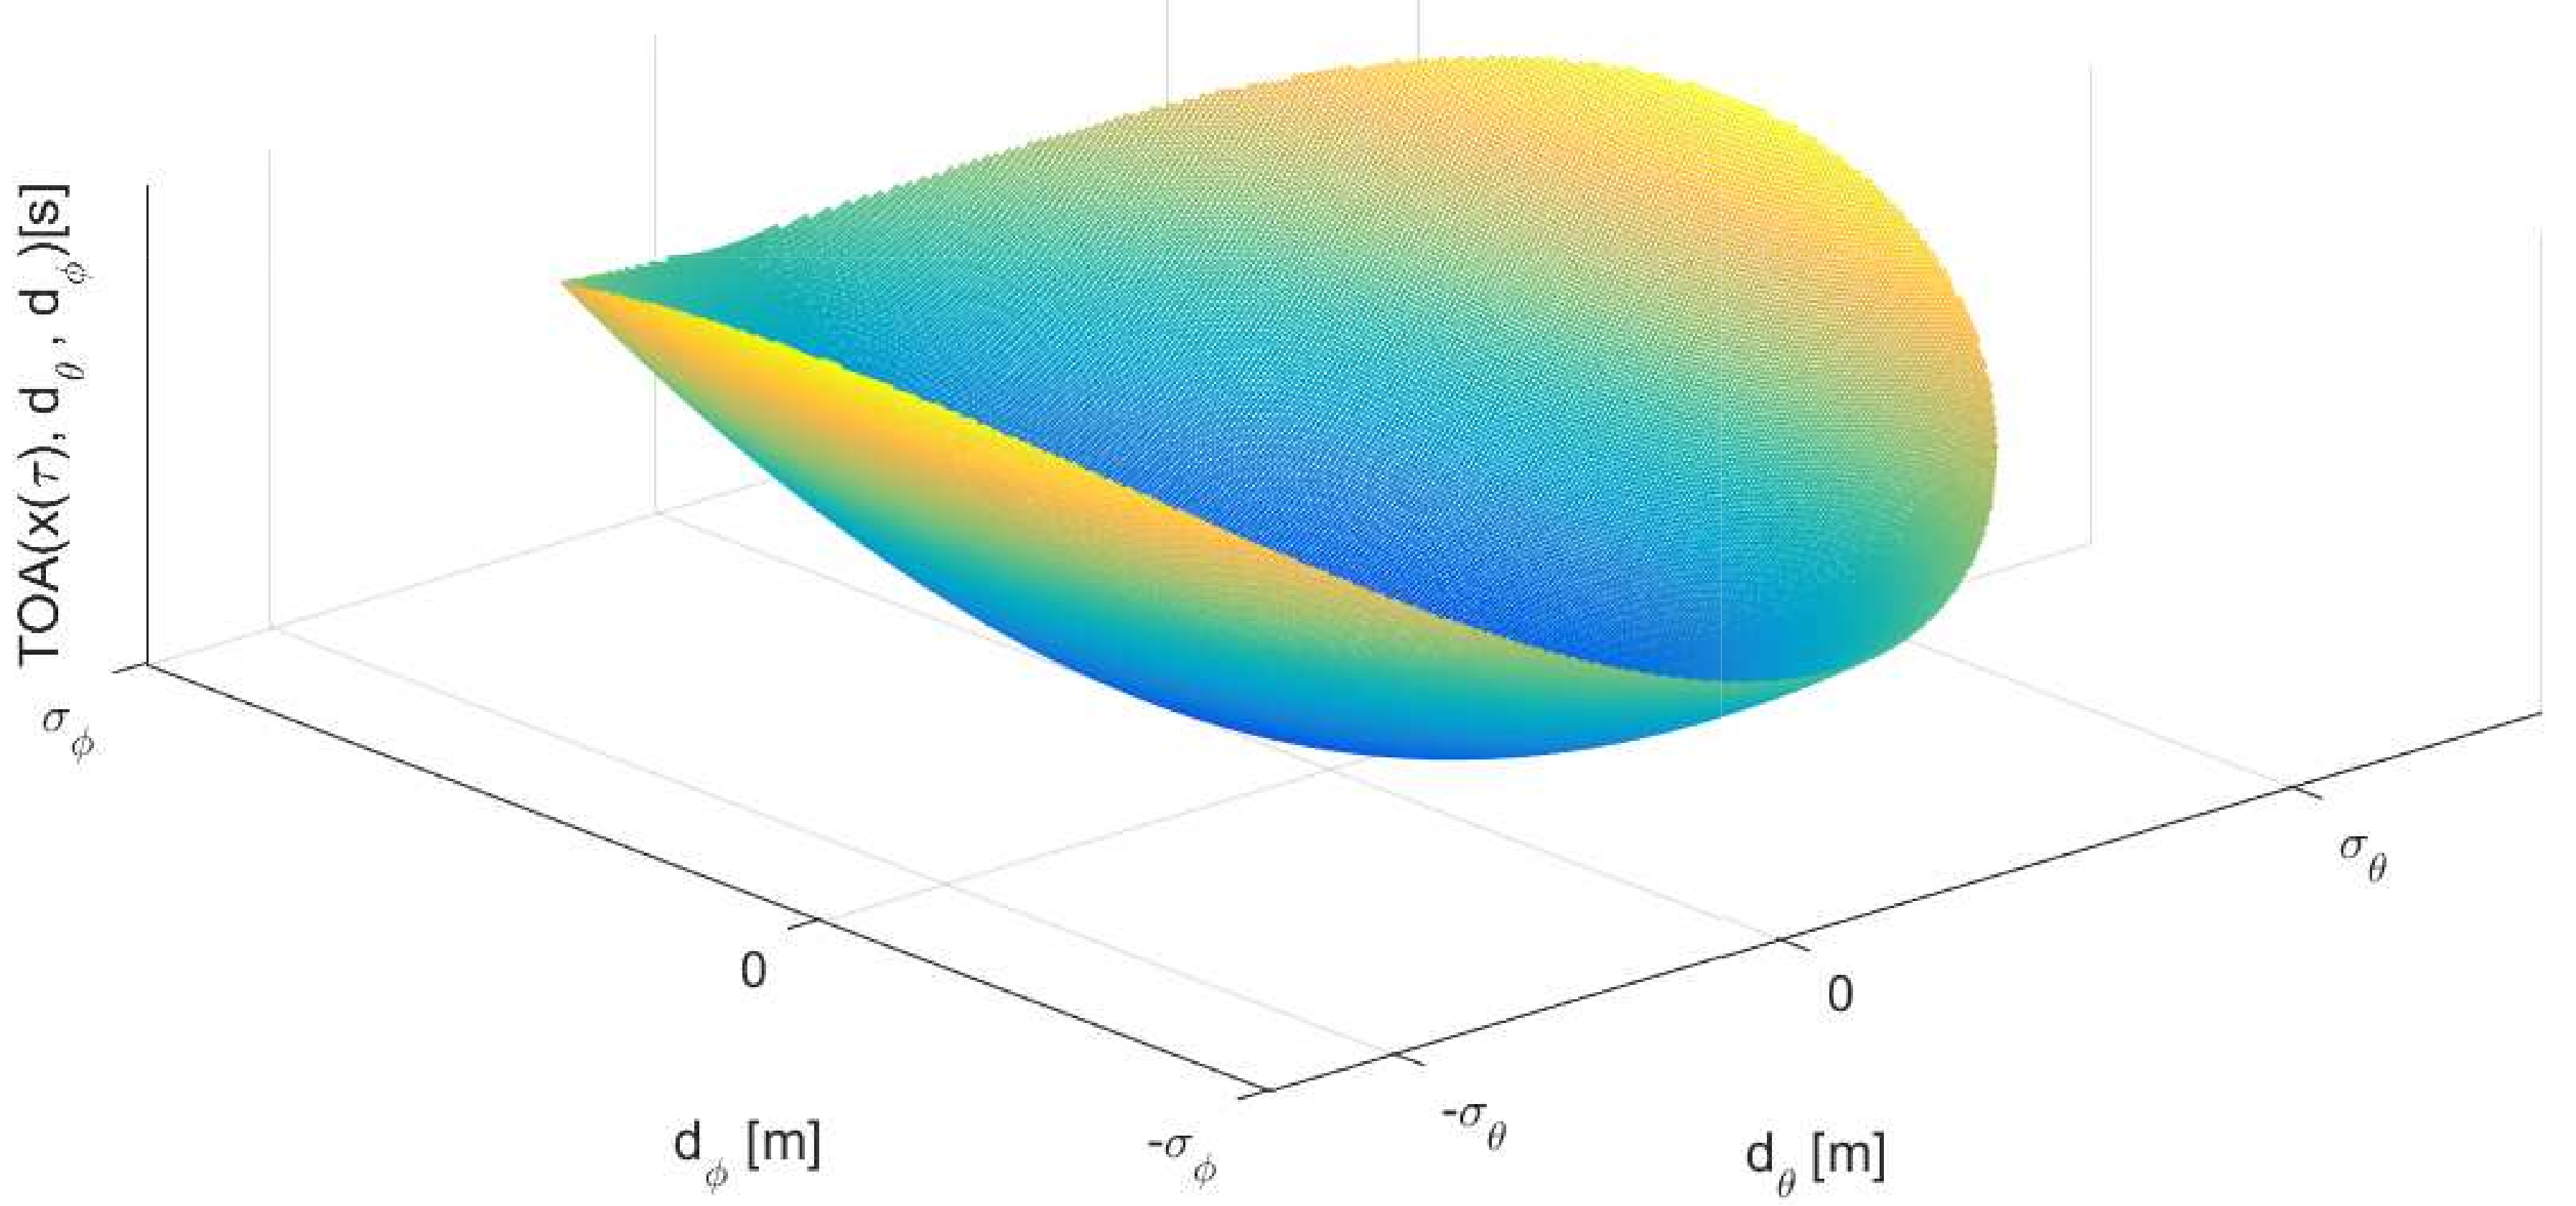
\includegraphics[width=0.9\linewidth]{\FIGDIR/TE016EllipsoidCutTimeOfArrival} 
            \caption{Time of arrival.}
            \label{fig:intruderTimeOfArrival}
        \end{subfigure}
        \caption{Properties for one elliptic cone slice. }
        \label{fig:propertiesEllipticConeSlice}
    \end{figure}

\subsection{(W) Moving Constraints}\label{s:MovingVirtualConstraints}
TODO new section look to Storm scenario structure

The algorithm used for intersection selected based on:\citep{bentley1979algorithms} the selected algorithm  \emph{Shamos-Hoey} \cite{shamos1976geometric}.
